\documentclass[10pt]{article}
\usepackage{arxiv}
\usepackage[T1]{fontenc}
\usepackage{amsmath,amssymb,booktabs,tabularx,graphicx}
\usepackage[numbers]{natbib}
\usepackage[hidelinks]{hyperref}
\usepackage{url}
\renewcommand{\shorttitle}{Radial adaptation under a compute constraint}
\renewcommand{\headeright}{Evidence report}
\renewcommand{\undertitle}{Research report; adaptive benefit not established}
\title{Separating Radial Structure from Adaptive Gating in Learned Dynamics:\\A Specification, Falsification Protocol, and Compute-Limited Study}
\author{Anonymous research draft}
\date{21 October 2026}
\begin{document}
\maketitle
\begin{abstract}
A physics-structured predictor can outperform a generic baseline without demonstrating that its adaptive component is useful. We examine this distinction for the RIPII radial-mixture model, which combines two history-conditioned central-force experts using a bounded scene-dependent gate. Earlier development results remain inconclusive because training adequacy was not established. We specify a new comparison against independently trained fixed gating, graph, pooling, and Transformer predictors, together with a within-checkpoint gate intervention. The protocol requires six independent data-generation blocks per domain, two nested initialization seeds, validation-only hyperparameter selection, and explicit training-adequacy checks before test access. Its implementation passed ten original CPU numerical tests and full-horizon CUDA backward and checkpoint-replay checks for all five models. A measured cost profile then rejected the 140-fit matrix under the authorized four allocated GPU-hour budget. No comparison training or test evaluation occurred. We report the model, mathematical guarantees and limitations, protocol, retained failure evidence, and an engineering investigation of execution overhead. These results establish an executable specification and a concrete feasibility limitation, not a positive scientific result for adaptive gating.
\end{abstract}
\keywords{learned dynamics \and adaptive gating \and mechanism controls \and reproducibility \and compute-constrained evaluation}

\section{Introduction}
The research question is whether scene-dependent mixing of two radial force experts improves held-out trajectory prediction beyond the same radial architecture with a fixed mixture. The distinction matters because geometric structure, integration rules, information access, and optimization can each improve a model independently of adaptation. A comparison against a generic graph predictor alone cannot identify the adaptive contribution.

The working hypothesis is precise: under the declared synthetic springs and charged-particle distributions, adequately trained adaptive radial prediction reduces mean paired 64-step position error by at least two percent relative to independently trained fixed radial prediction in both domains. A stronger mechanism claim additionally requires an advantage over replacing each trained adaptive gate by its training-set mean. This claim is falsifiable by adequately trained controls that match or outperform the adaptive predictor, by inadequate precision, or by failure of the intervention requirement.

The prior radial-mixture v3 study is retained as \texttt{INCONCLUSIVE\_UNDERTRAINED}. Its descriptive rankings are not converted into confirmatory evidence. The new study is a separate identity, \texttt{RIPII-RADIAL-ADAPTATION-v1}, with fresh generator blocks and a protected evaluation boundary. Its question remains unresolved because measured execution cost prevented training. This report does not claim perfection, state-of-the-art performance, real-world utility, or a new physical law.

\section{Related Work and Contribution Boundary}
Interaction Networks explicitly model objects and relations for dynamical prediction \citep{battaglia2016}. NRI jointly infers latent interactions and predicts dynamics from observations \citep{kipf2018}; the present experiments use its retained springs and charged-particle simulator implementation, not a reproduction of published NRI scores. EGNNs provide an established route to geometric equivariance \citep{satorras2021}. These precedents rule out describing relational modeling or invariant-to-vector updates as new by themselves.

NIIP instead represents relational constraints through learned energy functions and test-time trajectory optimization \citep{comas2023}. Our direct autoregressive predictor does not implement that inference mechanism. In particular, a velocity-dependent central force should not be described as an energy-conserving potential model without an additional derivation.

The contribution pursued here is a controlled test of adaptation within a specified radial predictor. The listed baselines are strong matched controls from this project's history, not a comprehensive current state-of-the-art suite. NRI, EGNN, potential-based methods, and task-specific analytic estimators remain relevant external comparisons before a broad superiority claim. No priority claim for the two-expert gate is made.

CUDA graph execution can reduce repeated host dispatch overhead for static workloads \citep{cuda2021}. Its applicability must be measured: a software optimization is neither a novel dynamics model nor evidence that the scientific hypothesis is true.

\section{Problem Formulation}
A scene contains $N=5$ objects. Each observed state is
$x_{t,i}=(p_{t,i},v_{t,i})\in\mathbb{R}^{4}$, with two-dimensional position and velocity. The input history is
$X\in\mathbb{R}^{B\times 8\times5\times4}$ and the target forecast is
$Y\in\mathbb{R}^{B\times64\times5\times4}$. Coordinates and velocities from the simulator are divided by five; these are normalized simulator units, not SI measurements. The observation interval is $\Delta t=0.05$.

The predictor receives past states only. Ground-truth interaction edges are retained in dataset artifacts for provenance but never supplied as model inputs. The forecast is autoregressive after the observed context. The finite history need not identify a unique underlying interaction law: observationally equivalent histories can require different future forces. Therefore prediction error is the endpoint; recovery of physical parameters is not claimed.

The optimization objective at curriculum horizon $H$ is
\begin{equation}
 \mathcal{L}_H(\theta)=
 \frac{1}{BH N4}\sum_{b=1}^{B}\sum_{h=1}^{H}\sum_{i=1}^{N}
 \left\|\widehat{x}_{b,h,i}-x_{b,h,i}\right\|_2^2.
\end{equation}
The sum notation includes the four state components through the squared norm. Evaluation uses position only:
\begin{equation}
 {\rm RMSE}_p=
 \sqrt{\frac{1}{B\,64\,N\,2}
 \sum_{b,h,i}\|\widehat{p}_{b,h,i}-p_{b,h,i}\|_2^2}.
\end{equation}
Thus training and selection objectives differ explicitly: training weights all normalized state coordinates equally, while checkpoint selection minimizes validation position RMSE.

\section{Complete Radial Model Specification}
\subsection{History features}
For every ordered pair $i\ne j$, define relative displacement $r_{ij}=p_i-p_j$, relative velocity $u_{ij}=v_i-v_j$, clipped distance
$d_{ij}=\max(\|r_{ij}\|_2,10^{-4})$, radial speed
$s_{ij}=r_{ij}^{\mathsf T}u_{ij}/d_{ij}$, and relative speed
$q_{ij}=\|u_{ij}\|_2$. Concatenating $(d,s,q)$ over eight observed times yields 24 inputs per pair. A two-linear-layer MLP with SiLU hidden activation maps $24\to64\to64$ to produce $e_{ij}$.

For each object and spatial axis $a$, concatenate the eight observed $(p_{i,a},v_{i,a})$ pairs. An MLP maps $16\to32\to32$ to produce the axis embedding $z_{i,a}$. Both embeddings are computed once per forecast and held fixed while the predicted state evolves.

\subsection{Experts and gate}
At each forecast step, form
\begin{equation}
 \xi_{ij}=[e_{ij},d_{ij},\min(d_{ij}^{-1},100),s_{ij},q_{ij}]\in\mathbb{R}^{68}.
\end{equation}
Two independent MLPs map $68\to64\to1$; their outputs are bounded by $\tanh$, giving $f^A_{ij},f^B_{ij}\in[-1,1]$.

The scene statistic vector contains mean and population standard deviation of directed-pair distance, mean absolute radial speed, and mean object speed. Concatenate it with the mean pair embedding to obtain 68 gate inputs. A $68\to64\to1$ MLP followed by a sigmoid gives
\begin{equation}
 g=0.05+0.90\,\sigma(G([\overline{e},{\rm stats}])).
\end{equation}
The adaptive coefficient is shared across all pairs in a scene at that forecast step. The fixed model sets $g=0.5$. It retains the gate module in serialization, but the gate parameters are inactive; equal stored parameter counts do not imply equal effective capacity.

The pair acceleration contribution is
\begin{equation}
 a^{\rm pair}_{ij}=20\,[g f^A_{ij}+(1-g)f^B_{ij}]\frac{r_{ij}}{d_{ij}}.
\end{equation}
An axis-shared $34\to32\to1$ MLP receives $[z_{i,a},p_{i,a},v_{i,a}]$ and gives
$a^{\rm wall}_{i,a}=20\tanh(W([z_{i,a},p_{i,a},v_{i,a}]))$. Total acceleration is the sum over senders plus this boundary term.

\subsection{Integration, initialization, and complexity}
The update is semi-implicit Euler:
\begin{equation}
 v_{t+1,i}=v_{t,i}+\Delta t\,a_{t,i},\qquad
 p_{t+1,i}=p_{t,i}+\Delta t\,v_{t+1,i}.
\end{equation}
The output linear layers of both experts and the boundary head start at zero. Consequently the initial predictor is constant velocity, while the gate is initially unidentifiable from prediction: both expert outputs coincide. Standard module initialization is retained for the other layers. No auxiliary gate loss or supervised edge objective is used.

For width $w$, pair computation is $O(BHN^2w^2)$ and stored unrolled activations are $O(BHN^2w)$ up to layer-dependent constants. The implementation explicitly fixes $N=5$ through its receiver/sender buffers; variable-size generalization is not demonstrated. The adaptive model contains 21,956 stored and gradient-active parameters. Fixed radial stores the same number but has 17,475 gradient-active parameters in the qualification check.

\subsection{What is and is not guaranteed}
Under pair reversal, both $r$ and $u$ change sign. Distance, radial speed, and relative-speed history remain unchanged, so paired expert coefficients match. The shared scene gate also matches. Hence $a^{\rm pair}_{ij}=-a^{\rm pair}_{ji}$, and the sum of internal pair accelerations is zero up to numerical error. This is an internal-force identity under the equal-mass interpretation. The external boundary term can change total momentum.

Central direction alone does not imply energy conservation: the coefficients depend on velocity and history and need not derive from a scalar potential. Semi-implicit Euler is not exact dynamics. The learned axis boundary term does not guarantee arbitrary rotational equivariance. These limits prevent extending a numerical momentum check into a claim of general physical correctness.

\section{Controls and Identifiability}
The primary comparator is a separately initialized and trained fixed-radial model with the same two experts, history encoders, boundary term, and integration rule. It isolates the trainable gate only imperfectly: the optimization path and effective parameter count also differ.

A second comparison intervenes on the selected adaptive checkpoint. The replacement gate is its mean over training scenes and forecast steps. Test observations never determine this constant. This intervention retains the trained experts and removes scene-dependent gate variation, but can create an off-training-distribution internal representation. It is therefore a diagnostic requirement in addition to, not a substitute for, independently trained fixed gating.

The generic controls are the retained graph, global-pool, and Transformer implementations, each receiving the same eight-frame state history and 64-step objective. Widths are chosen by the frozen search grid to minimize stored parameter-count difference. Qualification records 23,296 parameters for graph, 21,796 for pooling, and 22,756 for Transformer. The graph and pooling implementations use distance-threshold interactions; the Transformer has two encoder layers, four attention heads, zero dropout, and a feed-forward width twice its hidden width. These are project controls, not verified reproductions of external published baselines.

\section{Prospective Experimental Protocol}
\subsection{Data and protected boundary}
The two domains are springs and charged particles from the pinned NRI simulator. The exact source and upstream license are vendored in the retained package. Each fit uses 512 training scenes and 128 validation scenes. Each test regime would use 128 scenes. Sampling uses 50 simulator steps per observation and retains 72 observations. Every saved scene must have the declared shape and finite values.

Calibration uses generator block 5100011 and initialization seed 61001. Main blocks are 5200011, 5300021, 5400031, 5500041, 5600051, and 5700061; nested initialization seeds are 62003 and 63001. A dataset seed is $100b+c_d+c_s+c_r$, where domain offsets are 0/50, split offsets are 1/2/3, and regime offsets are 0/10/20/30. This makes the declared identities disjoint; it is not a proof of all possible forms of leakage.

The standard regime uses upstream defaults. Strong interaction uses strength 0.15 for springs and 1.5 for charged particles; fast motion uses velocity norm 0.75; noisy observations use noise variance parameter 0.01. The original simulator semantics govern these parameters. Regime changes are test-only. Test datasets may be generated only after every selected main fit passes adequacy and the selection manifest is frozen.

\subsection{Training and adequacy}
Two learning rates, $10^{-3}$ and $3\times10^{-4}$, are calibrated independently per domain and model using eligible validation performance. This gives $2\times5\times2=20$ calibration fits; the main matrix contains $2\times6\times2\times5=120$ fits.

Training uses AdamW, weight decay $10^{-4}$, batch size 16, and global gradient-norm clipping at 1.0. A CPU generator selects scenes and valid temporal windows. Curriculum horizons are 1, 2, 4, 8, 16, and 32 for consecutive 500-update stages, followed by horizon 64. Validation occurs every 500 updates using the full 64-step forecast. A plateau scheduler multiplies the learning rate by 0.5 after patience 2, with minimum $3\times10^{-6}$.

No fit is eligible before 6,000 updates. The maximum is 16,000. At least five full-horizon validation records are required. Both training and validation best-so-far position errors must improve by no more than one percent over the final four checks, and the selected checkpoint's training position RMSE must be at most 75 percent of constant velocity on the same training scenes. Only checkpoints trained at horizon 64 can be selected. The selected checkpoint is reloaded and its metrics recomputed.

These conditions reject important forms of undertraining, but do not prove global optimality: a stalled poor optimizer can plateau, and finite thresholds are conventions. Failure of any required fit blocks test access. No failed seed is silently replaced.

\subsection{Inference and decision rules}
For each domain and generator block, average error over the two nested initialization seeds before comparing methods. The generator block, not a forecast frame or an optimization seed, is the independent unit. Define block gain $G_b=(R_b-C_b)/R_b$ and log error ratio $L_b=\log(R_b/C_b)$ for reference $R$ and candidate $C$.

The one-sided paired sign-permutation test enumerates all $2^6$ sign assignments to the six $L_b$ values. This test relies on the relevant exchangeability/symmetry assumption under its null; independent simulation blocks alone do not prove that assumption. Holm adjustment covers the two primary domain comparisons. Adaptive benefit requires mean gain at least two percent, positive gain in every block, and adjusted $p\le0.05$ in both domains. The mechanism diagnostic also requires at least two percent mean gain and positive gains in every block against the training-mean gate intervention.

Separate gates require at least five percent mean gain against each generic baseline, with every block positive, and no more than five percent regression in any OOD block against the trained comparators. Passing the adaptive primary gate does not automatically pass these stronger gates. Raw per-scene and per-horizon errors and predictions are retained for replay. With six independent units, inference remains coarse; uncertainty must be interpreted within this synthetic scope.

\section{Observed Results}
\subsection{Engineering qualification and cost refusal}
The new study passed 14 local control tests, ten original hosted CPU numerical tests without skips, and CUDA full-horizon backward/checkpoint-replay checks for all five models. These are executable-model checks, not efficacy experiments.

\begin{table}[ht]
\centering\small
\caption{Measured full-horizon update time on the initial T4 worker. Maximum of five timed updates after warm-up; these are engineering measurements.}
\begin{tabular}{lr}\toprule Model & Seconds per update\\\midrule
radial\_mixture & 0.535\\
radial\_fixed & 0.470\\
graph & 0.999\\
simple\_pool & 0.959\\
transformer & 0.754\\
\bottomrule\end{tabular}\end{table}
Real calibration training-data generation took 278.41 seconds. The minimum-update matrix projection was 179.10 host-hours; the maximum-step estimate with safety margin was 721.99 host-hours. The allowed host duration was two hours because both allocated T4 devices count toward the four-GPU-hour cap.

The initial run elapsed 395.13 seconds. Including the 180-second export reserve, its conservative charge was 0.3195 allocated GPU-hours. Cloud spend was zero. The retained terminal status is cost-blocked, with zero of 140 comparison fits completed and no test data opened.


The minimum-update projection scales measured full-horizon training/validation timing to 6,000 updates across the matrix. It does not credit cheaper early curriculum stages and is not a mathematical lower bound. The maximum estimate includes data, evaluation, and a 1.5 safety factor. Neither projection guarantees adequate training. Their role is resource admission. No adaptive-versus-fixed effect size, ablation score, confidence interval, or positive test conclusion exists for this new study.

\subsection{Execution optimization investigation}
The engineering candidate removes repeated host-side tensor-value checks from the inner rollout, evaluates fixed-shape dense edge messages with explicit masks, and captures repeated CUDA training operations. Public entry checks and post-update finite checks remain necessary; diagnostics can be computed using the original model outside the timed training kernel. Dense masking must preserve the dynamic distance threshold and its gradient behavior.

Qualification compares original and optimized outputs and parameter gradients at horizons 1, 8, and 64 after nonzero head perturbations; zero-initialized heads alone would be a vacuous test. It additionally checks edge-threshold cases, optimizer updates, serialization, invalid input rejection, and captured-versus-eager updates with changing data. Predeclared numerical tolerances are absolute $2\times10^{-5}$ and relative $2\times10^{-4}$; checkpoint replay is exact. A mismatch rejects equivalence rather than authorizing relaxed tolerances after inspection.
The amended execution candidate passed all five model fixtures at the scientific weight decay $10^{-4}$, including a captured tensor learning-rate change from 0.001 to 0.0005. The initial optimizer fixture at default weight decay 0.01 is retained as a separate earlier attempt.

The largest absolute parameter-gradient and ordinary optimizer-update differences were 2.38e-07 and 3.99e-07, respectively. Captured-versus-eager optimizer updates and serialized forecast replay were exact in the tested cases. These finite fixtures are not a proof over every input or an independently reproduced training campaign.

\begin{table}[ht]\centering\small\caption{Protocol-matched captured training-step measurements. Maximum of seven timed updates; engineering fixtures only.}\begin{tabular}{lr}\toprule Model & Seconds per update\\\midrule
radial\_mixture & 0.0537\\
radial\_fixed & 0.0482\\
graph & 0.0600\\
simple\_pool & 0.0621\\
transformer & 0.0566\\
\bottomrule\end{tabular}\end{table}
The update-only minimum-step extrapolation is 13.10 host-hours, excluding data generation, validation, graph capture, serialization, and safety reserve. This remains above the remaining authorized host time; the full study was not admitted. All three numerical attempts together charge 0.5748 allocated GPU-hours, including export reserves, with zero cloud spend.

\begin{figure}[ht]
\centering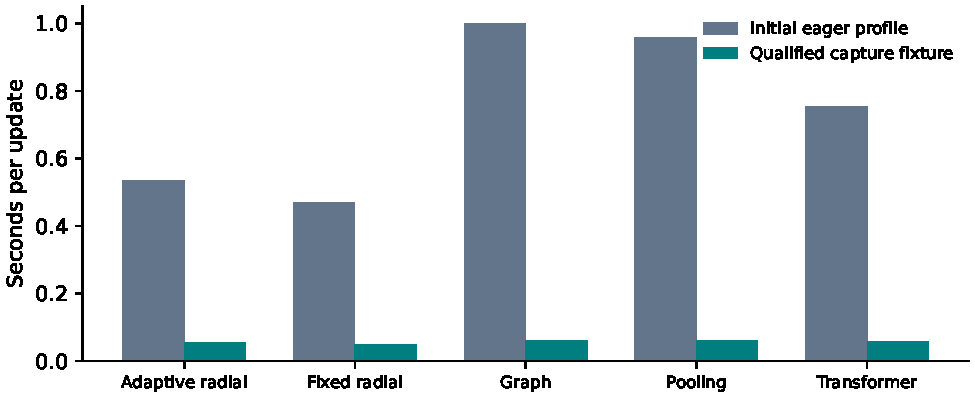
\includegraphics[width=0.95\linewidth]{timing.pdf}
\caption{Descriptive update timings from separate Kaggle T4 runs. The plotted maxima use five measured initial updates and seven captured updates. Hardware state, fixture setup, and timing boundaries differ; this is not a paired speedup estimate or an efficacy result.}
\end{figure}

\section{Failure Analysis and Adversarial Audit}
The central unresolved issue is identifiability of adaptive value. A radial model can gain through its geometric prior while a fixed mixture provides the same forecast quality. Expert label exchange leaves the mixture unchanged after complementing the gate; equal experts make the gate irrelevant. Gate variance alone therefore cannot establish a causal or physical interpretation.

The principal experiment-design defect is feasibility. A 140-fit convergence-aware matrix is disproportionate to a four-GPU-hour budget with the measured implementation. This was discovered before protected outcomes, and the refusal is retained. Reducing steps after observing this refusal would recreate the original adequacy problem. Reducing domains, seeds, or comparators would change the scientific question and requires a separately declared study.

Other material limitations are the fixed object count, synthetic data, incomplete effective-capacity matching, lack of wall-time matching across all controls, coarse independent-unit inference, unproven latest-baseline coverage, and incomplete independent reproduction. The repository's flaw register maps each issue to its cause, repair, and required acceptance evidence. Passing software checks does not close these scientific gaps.

\section{Discussion and Limitations}
This work has established neither that adaptation helps nor that it is useless. The new study has no test outcomes. The earlier undertrained study cannot resolve the missing comparison, and a faster implementation cannot supply an effect estimate by itself.

The next experiment is justified only if measured end-to-end cost fits the remaining authorization and equivalence checks pass. Otherwise the honest endpoint is an unresolved hypothesis with a documented feasibility limit. A future narrower question can be worthwhile, but its claims must match its domains, baselines, and independent units. Real-world performance, stability over longer horizons, object-count scaling, calibrated uncertainty, and physical-parameter recovery remain untested.

The finite engineering fixtures do not prove functional equality for every possible input. Conversely, a numerical mismatch may reflect reduction order or a true bug; it must be explained before substituting an implementation. Repeated attempts to obtain a passing benchmark would need a fixed development budget and preserved failures.

\section{Reproducibility and Release Status}
The reference source freeze, protocol, predecessor hashes, raw Kaggle archive, environment, per-model qualification records, cost profile, charge ledger, and failure trace are retained. The scientific output archive SHA-256 begins \texttt{9f7bdfcd5ae30fe7}; the source freeze begins \texttt{2904cd7cb3487219}. Full digests and artifact paths appear in the repository evidence manifest.

The original study and engineering probe use separate identities. Budget accounting carries prior charges forward and counts both allocated T4 devices even when one device executes the worker. Local heavy work was refused when resource admission failed. Cloud runs use free Kaggle only and no paid scaling.

The manuscript uses the retained user-supplied arXiv style without modifying its bytes. Its layout is not proof of arXiv acceptance. Authorship, affiliations, licensing of the whole release, and submission authorization are not inferred. This anonymous research draft is an evidence report, not a submission-ready positive-results paper.

\section{Conclusion}
A controlled adaptive-versus-fixed comparison requires adequate training and a mechanism-specific intervention. We implemented that comparison and verified its executable components, but measured cost prevented the experiment under its declared budget. The hypothesis remains untested in the new study. The defensible result is the exact model specification, preserved evidence boundary, and measured feasibility failure, together with a separately qualified attempt to reduce execution overhead. No unsupported positive conclusion is substituted for missing experiments.

\section*{AI Use}
AI assistance supported implementation, auditing, literature retrieval, and drafting. Retained artifacts determine numerical claims. Human authors remain responsible for scientific interpretation, attribution, licensing, and any submission.

\appendix
\section{Evidence and Acceptance Requirements}
A valid efficacy claim requires the chain: frozen protocol and source; complete calibration and main-fit inventory; passed adequacy records; frozen validation-only selections; raw protected predictions and targets; independent metric and statistical replay; and figures/tables regenerated from those records. None of the engineering checks replaces the missing trained-model portion of this chain.

The fixed-radial comparison, within-checkpoint gate intervention, generic-baseline gate, and OOD gate must be reported separately. A failure in one cannot be concealed by averaging it with a success in another. A missing comparison is reported as missing, not zero improvement.

\begin{thebibliography}{9}
\bibitem{battaglia2016} P. W. Battaglia, R. Pascanu, M. Lai, D. Rezende, and K. Kavukcuoglu. Interaction Networks for Learning about Objects, Relations and Physics. NeurIPS, 2016. \url{https://arxiv.org/abs/1612.00222}.
\bibitem{kipf2018} T. Kipf, E. Fetaya, K.-C. Wang, M. Welling, and R. Zemel. Neural Relational Inference for Interacting Systems. ICML, 2018. \url{https://arxiv.org/abs/1802.04687}.
\bibitem{satorras2021} V. Garcia Satorras, E. Hoogeboom, and M. Welling. E(n) Equivariant Graph Neural Networks. ICML, 2021. \url{https://arxiv.org/abs/2102.09844}.
\bibitem{comas2023} A. Comas-Massagu\'e et al. Inferring Relational Potentials in Interacting Systems. ICML, 2023. \url{https://arxiv.org/abs/2310.14466}.
\bibitem{cuda2021} V. Nguyen et al. Accelerating PyTorch with CUDA Graphs. PyTorch, 2021. \url{https://pytorch.org/blog/accelerating-pytorch-with-cuda-graphs/}.
\end{thebibliography}
\end{document}
